
\documentclass[11pt,a4paper]{article}
\usepackage{fontspec}
\usepackage{polyglossia}
\setdefaultlanguage{ukrainian}
\setotherlanguage{english}
\setmainfont{Liberation Serif}
\setsansfont{Liberation Sans}
\setmonofont{DejaVu Sans Mono}[Scale=0.82]
\usepackage[margin=2cm]{geometry}
\usepackage{amsmath,amssymb}
\usepackage{graphicx}
\usepackage{booktabs}
\usepackage{float}
\usepackage[font=small,labelfont=bf]{caption}
\usepackage{enumitem}
\setlist{itemsep=2pt,topsep=3pt}
\usepackage{xcolor}
\usepackage{tikz}
\usetikzlibrary{positioning,arrows.meta,fit}
\usepackage[hidelinks]{hyperref}
\usepackage{fancyhdr}
\pagestyle{fancy}\fancyhf{}\rhead{\small КП4: DQN у Acrobot-v1}\lhead{\small Основи глибокого навчання з підкріпленням}\cfoot{\thepage}
\renewcommand{\headrulewidth}{0.4pt}
\newcommand{\code}[1]{\texttt{#1}}

\begin{document}
\sloppy

\begin{titlepage}
\centering
{\large Основи глибокого навчання з підкріпленням (КПІ, ФІОТ, ІСТ, 2026)}\\[3cm]
{\LARGE\bfseries Комп'ютерний практикум № 4}\\[0.6cm]
{\Large Дослідження методу Deep Q-Network (DQN)\\ у середовищі Acrobot-v1}\\[1.5cm]
\begin{minipage}{0.8\textwidth}\small
\textbf{Мета роботи:} поглибити розуміння обраного методу глибокого навчання з підкріпленням, дослідити його нейромережеву архітектуру та вплив гіперпараметрів на процес навчання і поведінку агента.
\end{minipage}\\[2.5cm]
\begin{tabular}{rl}
Метод: & DQN (value-based, off-policy, model-free)\\
Реалізація: & Stable-Baselines3 2.x, PyTorch\\
Середовище: & Gymnasium \code{Acrobot-v1}\\
Експериментів: & 9 конфігурацій $\times$ 3 seed = 27 запусків по 60\,000 кроків\\
\end{tabular}\\[3cm]
Виконав(ла): \rule{6cm}{0.4pt}\\[0.5cm]
Київ, 2026
\end{titlepage}

\tableofcontents
\newpage

\section{Задача та середовище}

\textbf{Acrobot} — дволанковий маятник: верхня ланка закріплена шарніром, а привод є лише в шарнірі між ланками (недоактуована система). Агент має розгойдати систему так, щоб кінець нижньої ланки піднявся вище заданого рівня. Задача вимагає планування: одним «рухом» ціль недосяжна, потрібно накопичувати енергію серією узгоджених у часі дій.

\begin{table}[H]\centering\small
\begin{tabular}{p{3.6cm}p{12.4cm}}\toprule
Спостереження & \code{Box(6,)}, float32: $\cos\theta_1,\ \sin\theta_1,\ \cos\theta_2,\ \sin\theta_2,\ \dot\theta_1\in[-4\pi,4\pi],\ \dot\theta_2\in[-9\pi,9\pi]$ ($\theta_1$ — кут верхньої ланки від вертикалі, $\theta_2$ — кут нижньої відносно верхньої) \\
Дії & \code{Discrete(3)}: момент $-1$, $0$, $+1$~Н·м у середньому шарнірі \\
Винагорода & $-1$ за кожен крок, поки ціль не досягнута; $0$ на кроці досягнення цілі \\
Завершення (terminated) & висота кінця $-\cos\theta_1-\cos(\theta_1+\theta_2)>1$ \\
Обрізання (truncated) & 500 кроків (\code{TimeLimit}) \\
Критерій якості & середній дохід за епізод (дохід $=-$кількість кроків до цілі; $-500$ — ціль не досягнута); поріг «розв'язано» в Gymnasium — $-100$; додатково — частка успішних епізодів \\ \bottomrule
\end{tabular}
\caption{Опис середовища Acrobot-v1}
\end{table}

Винагорода прямо відповідає меті — дістатися цілі якомога швидше, — але є \emph{розрідженою}: поки агент випадково не підніме кінець ланки, всі епізоди дають однакові $-500$ і не містять інформації про напрямок покращення. Випадкова політика за 20 епізодів жодного разу не досягла цілі (усі $-500$).

\textbf{Різниця terminated / truncated.} Завершення через досягнення цілі — справжній термінальний стан: майбутня цінність дорівнює нулю. Обрізання через 500 кроків — штучне обмеження часу: стан не термінальний, тому в цілі TD-оновлення має залишатися оцінка продовження. Stable-Baselines3 враховує це автоматично (через \code{TimeLimit.truncated} у буфері).

\section{Метод Deep Q-Network}

\subsection{Ідея}
DQN \cite{mnih} — це Q-learning (див. КП3) з функцією цінності дій, апроксимованою нейромережею $Q_\theta(s,a)$. Табличний Q-learning непридатний для неперервного простору станів Acrobot, а мережа узагальнює між близькими станами. Метод \textbf{value-based} (навчається лише $Q$; політика — жадібна за $Q$), \textbf{model-free} (модель переходів не використовується) і \textbf{off-policy} (ціль відповідає жадібній політиці, а дані збирає $\varepsilon$-жадібна поведінка; тому можна повторно використовувати старий досвід).

\subsection{Оновлення параметрів}
Наївна заміна таблиці мережею нестійка: послідовні переходи сильно корельовані, а ціль оновлення залежить від тих самих параметрів, що оновлюються. DQN вирішує це двома механізмами:
\begin{enumerate}
\item \textbf{Буфер відтворення} (replay buffer) обсягом \code{buffer\_size} зберігає переходи $(s,a,r,s',d)$. Для кожного оновлення вибирається випадковий батч розміру \code{batch\_size}, що руйнує кореляції і дозволяє використати кожен перехід багато разів.
\item \textbf{Цільова мережа} $Q_{\theta^-}$ — копія основної, яка оновлюється лише кожні \code{target\_update\_interval} кроків ($\theta^-\leftarrow\theta$). Між оновленнями ціль «заморожена».
\end{enumerate}
Ціль і функція втрат для батча $B$:
\[
y=r+\gamma\,(1-d)\max_{a'}Q_{\theta^-}(s',a'),\qquad
L(\theta)=\frac{1}{|B|}\sum_{(s,a,r,s',d)\in B}\ell_{\delta}\bigl(Q_\theta(s,a)-y\bigr),
\]
де $d$ — ознака справжнього завершення, $\ell_\delta$ — функція Хубера (\code{smooth\_l1\_loss}), менш чутлива до великих TD-помилок, ніж MSE. Параметри оновлює оптимізатор Adam з кроком \code{learning\_rate}; норма градієнта обмежується значенням 10.

\subsection{Дослідження та режими роботи}
Під час навчання дія вибирається $\varepsilon$-жадібно: $\varepsilon$ лінійно зменшується від 1 до \code{exploration\_final\_eps} протягом частки \code{exploration\_fraction} загального числа кроків, далі лишається сталим. Під час оцінювання агент діє \textbf{детерміновано} (жадібно, $\varepsilon=0$), а мережа не оновлюється.

\subsection{Алгоритм (як реалізовано в SB3)}
\begin{enumerate}[label=\arabic*.]
\item Ініціалізувати $Q_\theta$, $Q_{\theta^-}\leftarrow Q_\theta$, порожній буфер.
\item На кожному кроці: вибрати $a$ $\varepsilon$-жадібно, виконати, записати $(s,a,r,s',d)$ у буфер.
\item Кожні \code{train\_freq}$=4$ кроки виконати \code{gradient\_steps} оновлень (тут $-1$ — стільки ж, скільки зроблено кроків, тобто 4): вибрати батч, обчислити $y$ і зробити крок Adam за $\nabla_\theta L$.
\item Кожні \code{target\_update\_interval} кроків: $\theta^-\leftarrow\theta$.
\end{enumerate}

\section{Нейромережева архітектура}

\code{MlpPolicy} DQN містить дві мережі однакової структури (рис.~\ref{fig:arch}): \textbf{Q-net} (оцінює $Q$, визначає дії, оновлюється градієнтом) і \textbf{Q-net target} (лише для обчислення цілі $y$). Вхід — 6-вимірний вектор спостереження без нормалізації, вихід — три числа $Q(s,a)$, по одному для кожної дії. Приховані шари — повнозв'язні з ReLU; вихідний шар лінійний, бо Q-значення можуть бути будь-якими дійсними (тут від'ємними, близько $-60\ldots0$).

\begin{figure}[H]\centering
\begin{tikzpicture}[scale=0.95, transform shape, node distance=0.55cm and 1.25cm, every node/.style={font=\small},
  box/.style={draw, rounded corners, minimum width=2.25cm, minimum height=0.9cm, align=center, fill=#1},
  box/.default=blue!8, >=Stealth]
\node[box=gray!10] (in) {Спостереження\\ $s\in\mathbb R^6$};
\node[box, right=of in] (h1) {Linear 6$\to$256\\ ReLU};
\node[box, right=of h1] (h2) {Linear 256$\to$256\\ ReLU};
\node[box=orange!15, right=of h2] (out) {Linear 256$\to$3\\ $Q(s,\cdot)$};
\draw[->] (in) -- (h1); \draw[->] (h1) -- (h2); \draw[->] (h2) -- (out);
\node[box=green!10, below=1.2cm of h2, minimum width=5.9cm] (tg) {Q-net target (та сама структура, ваги $\theta^-$)};
\draw[->, dashed] (h2.south) ++(0,-0.05) -- node[right, font=\scriptsize]{копія ваг кожні 250 кроків} (tg.north);
\node[right=0.6cm of out, align=left, font=\scriptsize] (pol) {дія $=\arg\max_a Q(s,a)$\\ (+$\varepsilon$-шум у навчанні)};
\draw[->] (out) -- (pol);
\node[below=0.25cm of tg, font=\scriptsize] {$y=r+\gamma(1-d)\max_{a'}Q_{\theta^-}(s',a')$};
\end{tikzpicture}
\caption{Архітектура Q-мережі DQN у базовій конфігурації (68\,355 параметрів).}\label{fig:arch}
\end{figure}

\begin{table}[H]\centering\small
\begin{tabular}{lll r}\toprule
Конфігурація & Приховані шари & Активація & Параметрів Q-net \\ \midrule
базова (RL Zoo) & 256, 256 & ReLU & 68\,355 \\
середня & 64, 64 & ReLU & 4\,803 \\
мала & 16 & ReLU & 163 \\ \bottomrule
\end{tabular}
\caption{Досліджені варіанти архітектури}
\end{table}

\section{Програмна реалізація}
\begin{itemize}
\item \textbf{Алгоритм:} Stable-Baselines3, клас \code{stable\_baselines3.DQN} \cite{sb3}; код алгоритму не змінювався.
\item \textbf{Базові гіперпараметри:} RL Baselines3 Zoo, файл \code{hyperparams/dqn.yml}, запис \code{Acrobot-v1} \cite{zoo}; ті самі значення наведено в картці навченої моделі \url{https://huggingface.co/sb3/dqn-Acrobot-v1} (результат $-72.1\pm6.4$ після $10^5$ кроків).
\item \textbf{Власні зміни та доповнення:}
  \begin{itemize}
  \item скрипт \code{cw4\_experiments.py}: серії експериментів з одним зміненим гіперпараметром відносно базової конфігурації, по 3 seed; паралельний запуск; журнал навчальних епізодів (\code{Monitor}); детерміноване оцінювання кожні 3\,000 кроків на 10 епізодах (\code{EvalCallback}); фінальне оцінювання кожної моделі на 50 епізодах із фіксованими seed; збереження моделей і метрик;
  \item ноутбук \code{DRL26\_CW4\_DQN\_Acrobot.ipynb}: зведені таблиці, криві навчання, діагностика невдалих запусків (жадібна vs $\varepsilon$-жадібна оцінка, розподіл дій), демонстрація поведінки агента (GIF, висота, дії, Q-значення);
  \item бюджет навчання скорочено з $10^5$ до $6\cdot10^4$ кроків через обмежені обчислювальні ресурси (2 ядра CPU, без GPU; ~3 хв на запуск).
  \end{itemize}
\end{itemize}

\section{Базова конфігурація та план експериментів}

\begin{table}[H]\centering\small
\begin{tabular}{lll}\toprule
Гіперпараметр & Значення & Призначення \\ \midrule
\code{learning\_rate} & $6.3\cdot10^{-4}$ & крок оптимізатора Adam \\
\code{batch\_size} & 128 & переходів в одному оновленні \\
\code{buffer\_size} & 50\,000 & обсяг буфера відтворення \\
\code{learning\_starts} & 0 & кроків до початку навчання \\
\code{gamma} & 0.99 & коефіцієнт дисконтування \\
\code{target\_update\_interval} & 250 & період копіювання ваг у цільову мережу \\
\code{train\_freq} / \code{gradient\_steps} & 4 / $-1$ & 4 оновлення на кожні 4 кроки середовища \\
\code{exploration\_fraction} & 0.12 & частка навчання, протягом якої $\varepsilon$ спадає \\
\code{exploration\_final\_eps} & 0.1 & кінцеве $\varepsilon$ \\
\code{net\_arch} & [256, 256] & приховані шари Q-мережі \\ \bottomrule
\end{tabular}
\caption{Базова конфігурація (RL Baselines3 Zoo)}
\end{table}

\textbf{Обґрунтування вибору гіперпараметрів для дослідження.} Обрано по одному параметру з кожного ключового компонента DQN: (1) \emph{оптимізація} — \code{learning\_rate}; (2) \emph{стабілізація цілі} — \code{target\_update\_interval}, головна відмінність DQN від наївного Q-learning з мережею; (3) \emph{апроксиматор} — архітектура \code{net\_arch}; (4) \emph{дослідження} — розклад $\varepsilon$. Значення взято по обидва боки від базового з кроком приблизно в 5–10 разів, щоб ефект був помітним на фоні шуму між seed.

\begin{table}[H]\centering\small
\begin{tabular}{p{3cm}p{4.8cm}p{7.6cm}}\toprule
Група & Варіанти (базове — жирним) & Гіпотеза \\ \midrule
Крок навчання & $10^{-4}$, $\mathbf{6.3\cdot10^{-4}}$, $3\cdot10^{-3}$ & малий — повільніше; великий — швидше, але нестабільніше \\
Цільова мережа & 10, \textbf{250}, 2000 & часте оновлення — «рухома ціль», нестабільність; рідке — повільне поширення цінностей \\
Архітектура & [16], [64,64], \textbf{[256,256]} & замала мережа не апроксимує $Q$; велика — надлишкова, повільніша \\
Дослідження & \textbf{(0.12, 0.1)}, frac = 0.5, $\varepsilon_{\text{final}}=0.01$ & довше дослідження — повільніший старт; мале $\varepsilon$ — ризик застрягти в поганій поведінці \\ \bottomrule
\end{tabular}
\caption{План експериментів (кожна конфігурація — 3 seed, 60\,000 кроків)}
\end{table}

\textbf{Показники.} \emph{Фінальний дохід} — середнє за 50 тестовими епізодами (жадібна політика, фіксовані seed), усереднене за 3 seed; \emph{std між seed} і \emph{найгірший seed} — стійкість до випадковості навчання; \emph{успішних} — частка тестових епізодів, що досягли цілі; \emph{крок досягнення $-100$} — перша проміжна оцінка вище порогу (середнє за seed, які його досягли); \emph{коливання} — середнє std останніх 5 проміжних оцінок одного запуску (стабільність наприкінці навчання).

\section{Хід експериментів і результати}

\begin{table}[H]\centering\small
\begin{tabular}{lrrrrlrr}\toprule
Конфігурація & Фін. дохід & std & Найгірший & Успішних & Поріг $-100$ & Коливання & Параметрів \\ \midrule
базова & $-$78.0 & 2.7 & $-$81.9 & 100\% & 30.0k (3/3) & 19.0 & 68\,355 \\
\texttt{lr}=$10^{-4}$ & $-$83.0 & 3.2 & $-$85.5 & 100\% & 25.0k (3/3) & 29.4 & 68\,355 \\
\texttt{lr}=$3\cdot10^{-3}$ & $-$77.4 & 3.7 & $-$81.6 & 100\% & 22.0k (3/3) & 34.9 & 68\,355 \\
target = 10 & $-$83.6 & 2.8 & $-$87.1 & 100\% & 20.0k (3/3) & 85.1 & 68\,355 \\
target = 2000 & $-$499.2 & 1.1 & $-$500.0 & 1\% & — & 45.8 & 68\,355 \\
{[16]} & $-$420.7 & 112.1 & $-$500.0 & 33\% & 16.5k (2/3) & 117.7 & 163 \\
{[64, 64]} & $-$80.0 & 2.4 & $-$82.9 & 100\% & 14.0k (3/3) & 11.2 & 4\,803 \\
expl.\,frac = 0.5 & $-$96.3 & 26.7 & $-$134.0 & 96\% & 19.0k (3/3) & 5.9 & 68\,355 \\
$\varepsilon_{\text{final}}=0.01$ & $-$135.3 & 78.2 & $-$245.9 & 87\% & 26.0k (3/3) & 16.1 & 68\,355 \\
\bottomrule
\end{tabular}
\caption{Зведені результати (3 seed на конфігурацію). Поріг: середній крок досягнення $-100$ (кількість seed, що досягли).}\label{tab:summary}
\end{table}

\begin{figure}[H]\centering
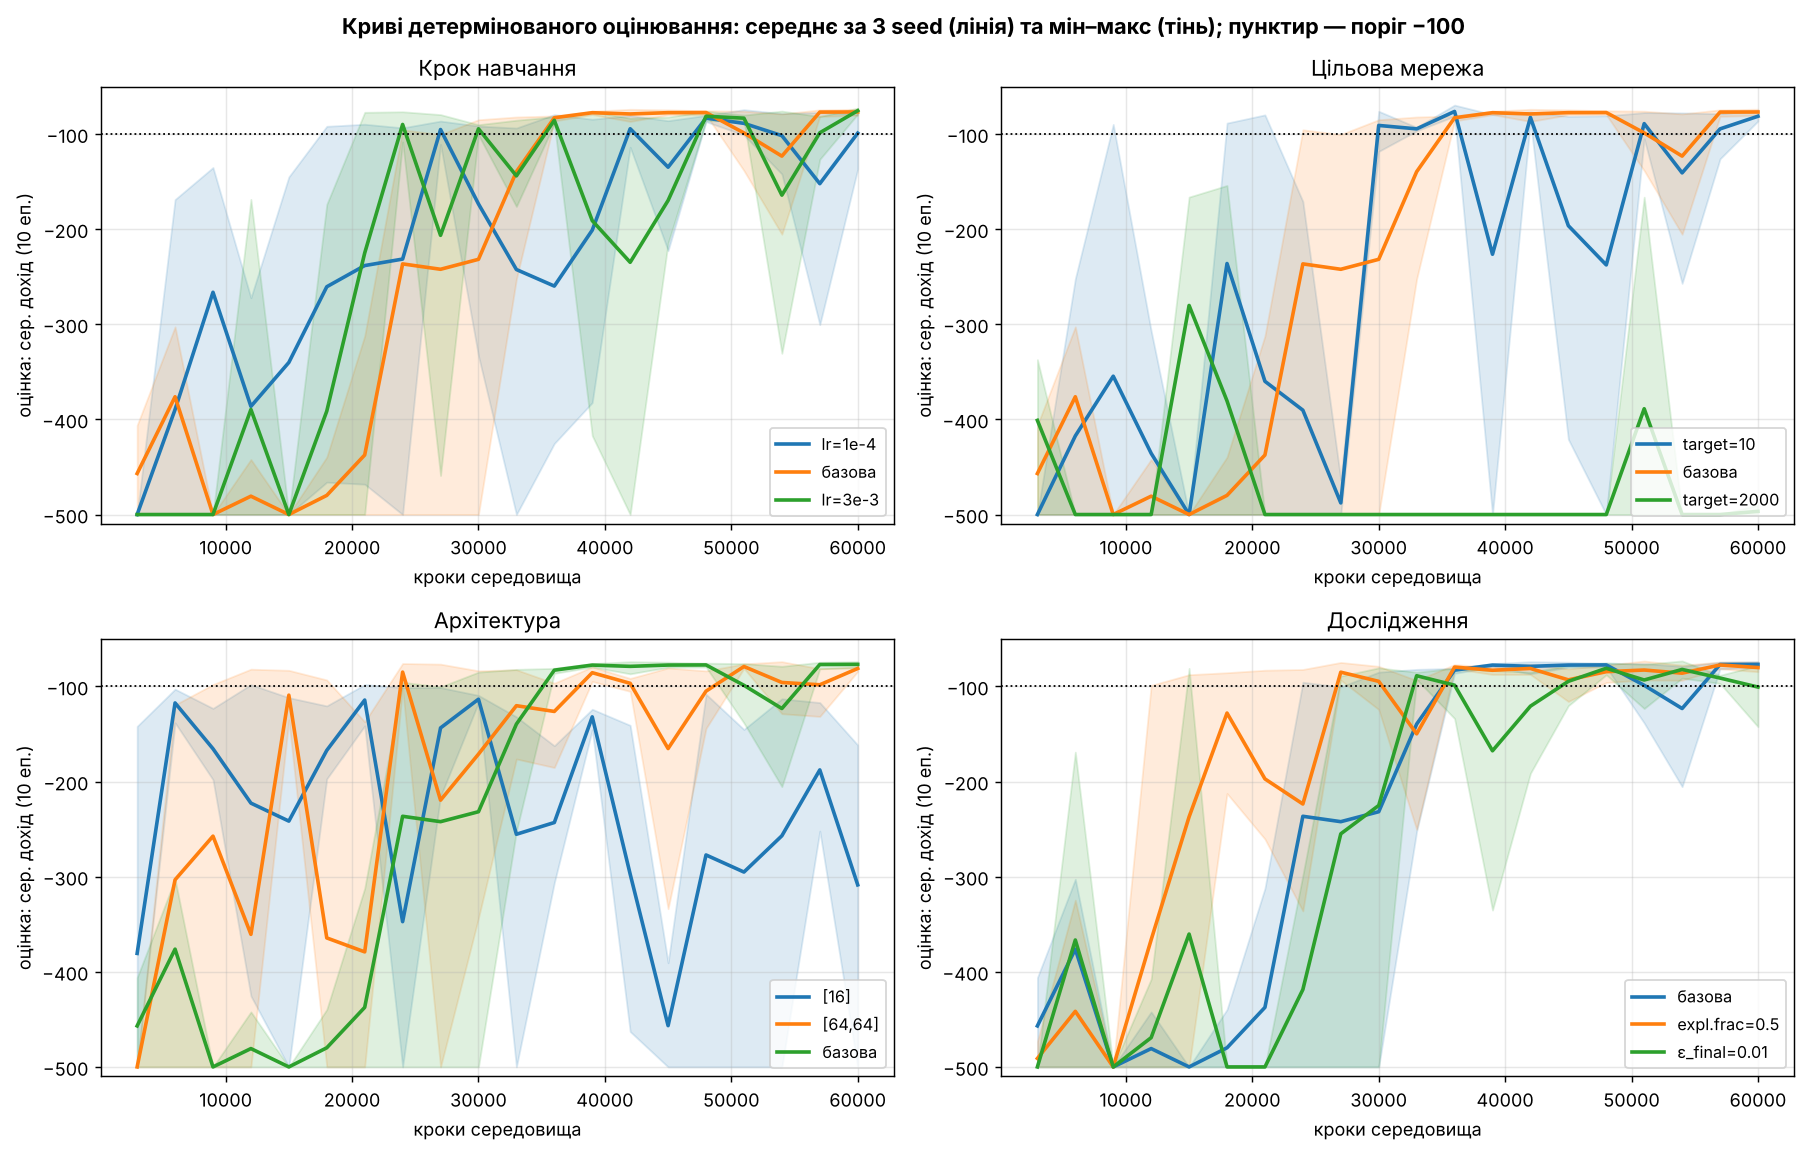
\includegraphics[width=\textwidth]{../fig_eval_curves.png}
\caption{Детерміноване оцінювання під час навчання (10 епізодів кожні 3\,000 кроків): середнє за 3 seed і мін–макс.}\label{fig:eval}
\end{figure}

\begin{figure}[H]\centering
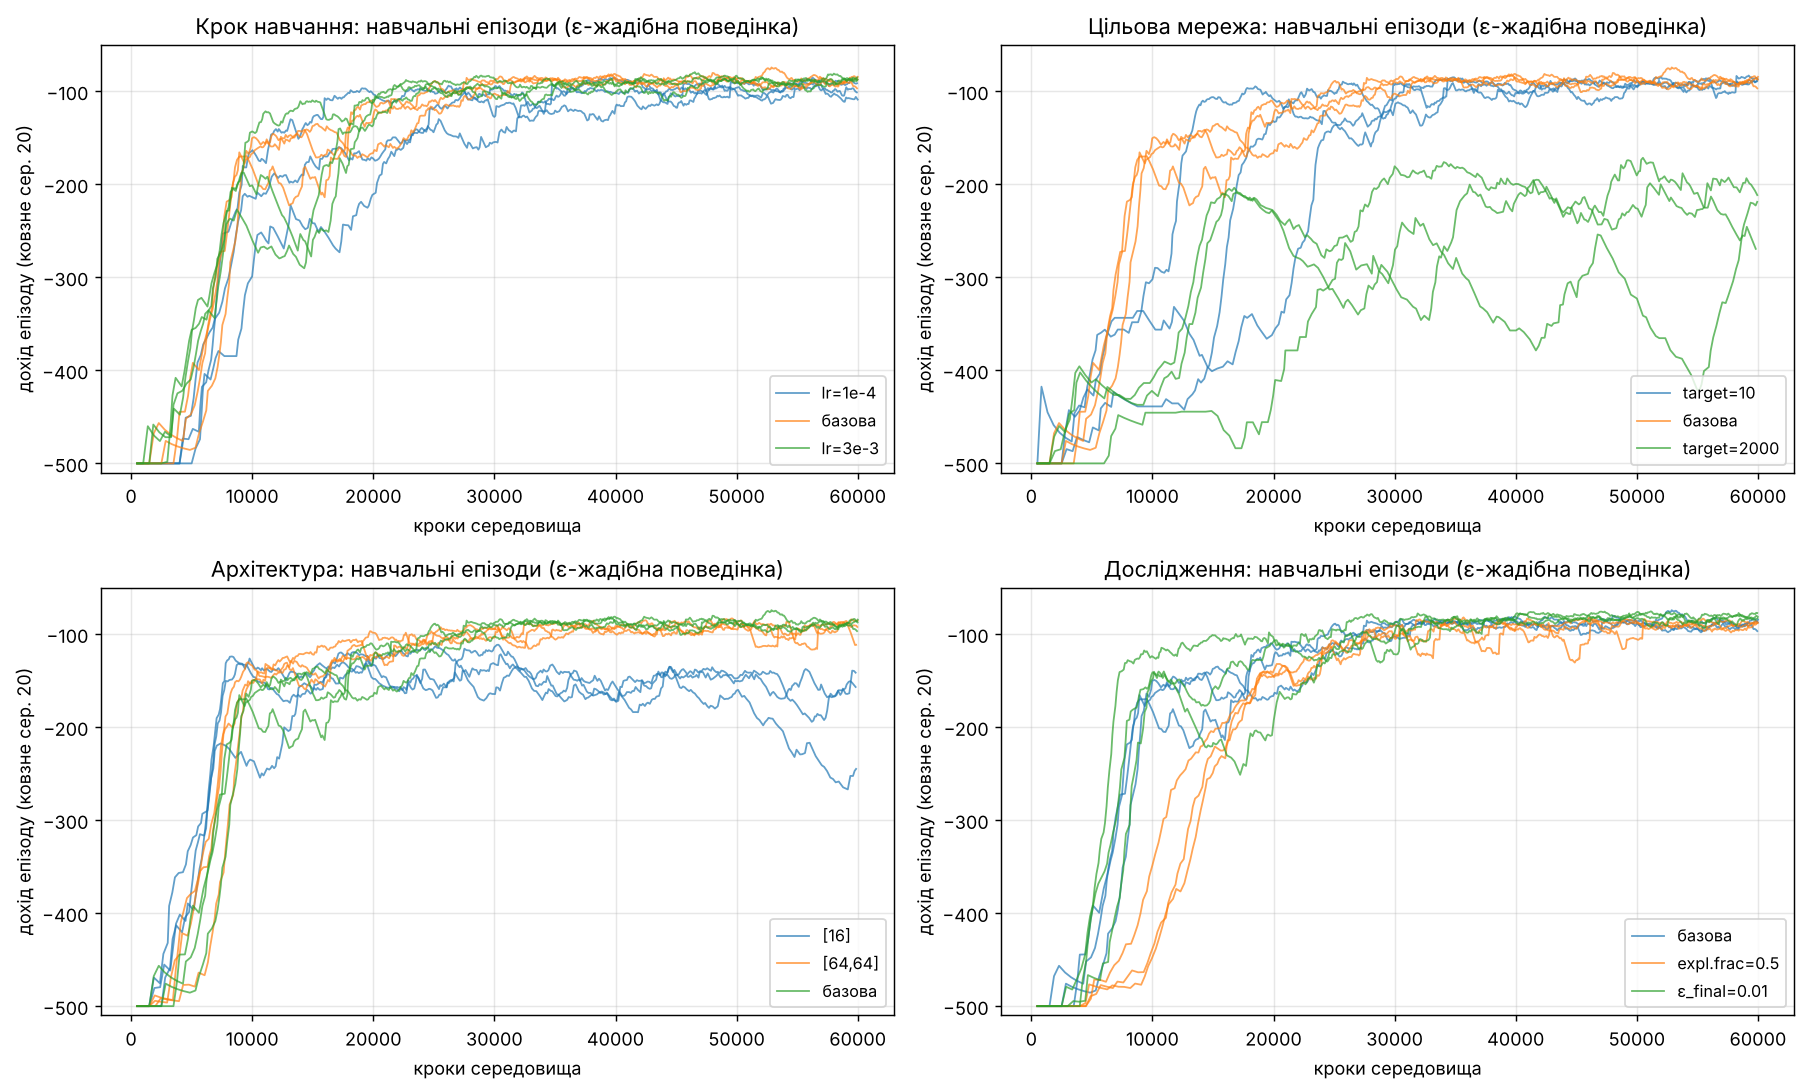
\includegraphics[width=\textwidth]{../fig_train_curves.png}
\caption{Доходи навчальних епізодів ($\varepsilon$-жадібна поведінка), ковзне середнє за 20 епізодами; кожна лінія — окремий seed.}\label{fig:train}
\end{figure}

\begin{figure}[H]\centering
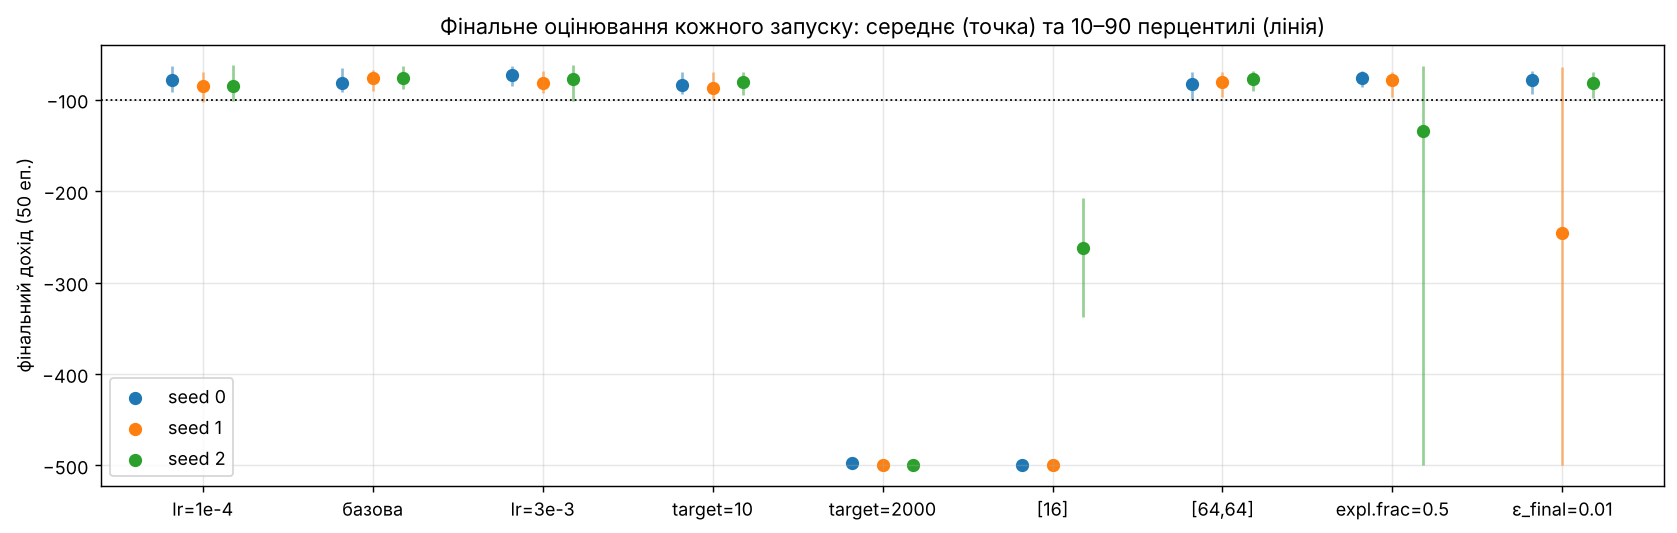
\includegraphics[width=\textwidth]{../fig_final.png}
\caption{Фінальне оцінювання кожного запуску (50 епізодів): середнє та 10–90 перцентилі.}\label{fig:final}
\end{figure}

\subsection{Експеримент 0: відтворення базової конфігурації}
\textbf{Мета:} перевірити, що готова реалізація з гіперпараметрами RL Zoo навчається в наших умовах. \textbf{Результат:} фінальний дохід $-78.0\pm2.7$, усі тестові епізоди успішні; поріг $-100$ перетнуто в середньому на 30-тисячному кроці. Це близько до опублікованого $-72.1\pm6.4$ при більшому бюджеті. Криві оцінювання (рис.~\ref{fig:eval}) до ~35 тис. кроків сильно коливаються: жадібна політика ще «перемикається» між вдалими та невдалими варіантами. Далі вона стабілізується біля $-80$.

\subsection{Експеримент 1: крок навчання}
\textbf{Мета:} оцінити чутливість до кроку Adam. \textbf{Результат:} усі три значення навчаються ($-83.0$, $-78.0$, $-77.4$). Більший крок раніше досягає порогу (22k проти 25–30k), але сильніше коливається наприкінці (35 проти 19–29). Менший крок повільніший, і за обмежений бюджет фінальний результат трохи гірший. \textbf{Спостереження:} у діапазоні $10^{-4}$–$3\cdot10^{-3}$ DQN доволі стійкий до \code{learning\_rate}: адаптивні кроки Adam, функція Хубера та обрізання градієнта обмежують величину оновлень. Відмінності фінального доходу порівнянні з розкидом між seed.

\subsection{Експеримент 2: період оновлення цільової мережі}
\textbf{Мета:} перевірити роль «заморожування» цілі. \textbf{Результат:} при оновленні кожні 10 кроків агент найшвидше досягає порогу (20k), але оцінки найнестабільніші: коливання 85, різкі провали кривих (рис.~\ref{fig:eval}) — ціль рухається разом із мережею. При 2000 агент за 60 тис. кроків не навчився ($-499$, жоден seed не досяг порогу): навчальні криві піднімаються лише до $-200$ і нестабільні. \textbf{Пояснення:} з цільовою мережею кожен період між оновленнями фактично реалізує одну ітерацію наближеної value iteration. При періоді 2000 за весь бюджет їх лише 30, а інформація про ціль має поширитися на горизонт ~80–100 кроків. Базове значення 250 — компроміс між стабільністю цілі та швидкістю поширення цінностей. Це найчутливіший з досліджених гіперпараметрів.

\subsection{Експеримент 3: архітектура мережі}
\textbf{Мета:} з'ясувати, яка ємність апроксиматора потрібна. \textbf{Результат:} [64,\,64] з у 14 разів меншою кількістю параметрів не поступається базовій ($-80.0$), найшвидше досягає порогу (14k), найстабільніша наприкінці (коливання 11) і обчислюється вдвічі швидше. [16] нестійка: два seed деградували до $-500$ (хоча на проміжних етапах досягали порогу), один — $-262$. \textbf{Спостереження:} базова [256,\,256] для цієї задачі надлишкова. Нижня межа ємності визначається не складністю динаміки, а потребою точно розрізняти близькі Q-значення дій (див. п.~\ref{sec:diag}).

\subsection{Експеримент 4: дослідження}
\textbf{Мета:} оцінити вплив тривалості та рівня дослідження. \textbf{Результат:} довша фаза спадання $\varepsilon$ (frac = 0.5) помітно уповільнює початок навчання (рис.~\ref{fig:train}): більше випадкових дій. Фінальний результат $-96.3$, один seed $-134$. Кінцеве $\varepsilon=0.01$ дало два добрі запуски ($-79$, $-81$) і один частково невдалий ($-246$), тому середнє $-135\pm78$. \textbf{Спостереження:} за малого дослідження буфер заповнюють схожі траєкторії, і помилки Q-мережі в рідко відвідуваних станах не виправляються. Базові параметри (0.12, 0.1) виявилися найнадійнішими.

\subsection{Діагностика невдалих запусків}\label{sec:diag}
Навчальні криві конфігурацій target = 2000 і [16] досягають $-150\ldots-250$, тоді як детерміноване оцінювання дає $\approx-500$. Фінальні моделі перевірено жадібно і з $\varepsilon=0.05$ (табл.~\ref{tab:diag}).

\begin{table}[H]\centering\small
\begin{tabular}{lcrrl}\toprule
Конфігурація & seed & Жадібно & $\varepsilon=0.05$ & Частки дій $-1$/0/$+1$ (жадібно) \\ \midrule
базова & 0 / 1 / 2 & $-81.5$ / $-74.0$ / $-74.7$ & $-89.0$ / $-79.0$ / $-83.5$ & 40/20/40, 44/9/47, 53/3/44 \% \\
target = 2000 & 0 & $-494.1$ & $-456.9$ & 0 / 98 / 2 \% \\
 & 1 & $-500.0$ & $-500.0$ & 100 / 0 / 0 \% \\
 & 2 & $-500.0$ & $-500.0$ & 0 / 0 / 100 \% \\
{[16]} & 0 & $-500.0$ & $-407.8$ & 0 / 0 / 100 \% \\
 & 1 & $-500.0$ & $-384.6$ & 0 / 100 / 0 \% \\
 & 2 & $-264.1$ & $-267.6$ & 15 / 28 / 57 \% \\
$\varepsilon_{\text{final}}=0.01$ & 1 & $-250.7$ & $-111.2$ & 8 / 0 / 91 \% \\ \bottomrule
\end{tabular}
\caption{Діагностика: у невдалих запусках жадібна політика вироджується в одну дію}\label{tab:diag}
\end{table}

У всіх невдалих запусках жадібна політика вибирає \emph{одну й ту саму дію майже в усіх станах} (постійний момент), тож маятник не розгойдується. Причина — малий «action gap»: у навченого агента різниця між Q найкращої та другої дії становить у середньому лише 0.6 при $|Q|\approx30$ (близько 2\%). Мережа має точно передати велику спільну цінність стану і водночас малу різницю між діями. Мала мережа або застаріла ціль цю різницю «губить», і $\arg\max$ визначається систематичною похибкою. Під час навчання $\varepsilon$-шум частково маскує дефект, тому навчальні криві виглядають кращими за реальну якість жадібної політики.

\subsection{Поведінка навченого агента}

\begin{figure}[H]\centering
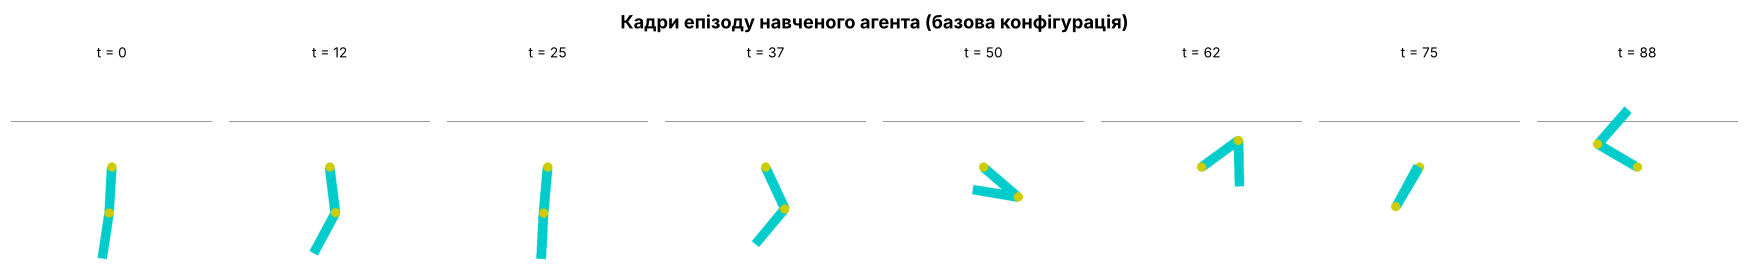
\includegraphics[width=\textwidth]{../fig_frames.png}
\caption{Кадри епізоду агента базової конфігурації (seed 0): ціль досягнута за 88 кроків.}
\end{figure}

\begin{figure}[H]\centering
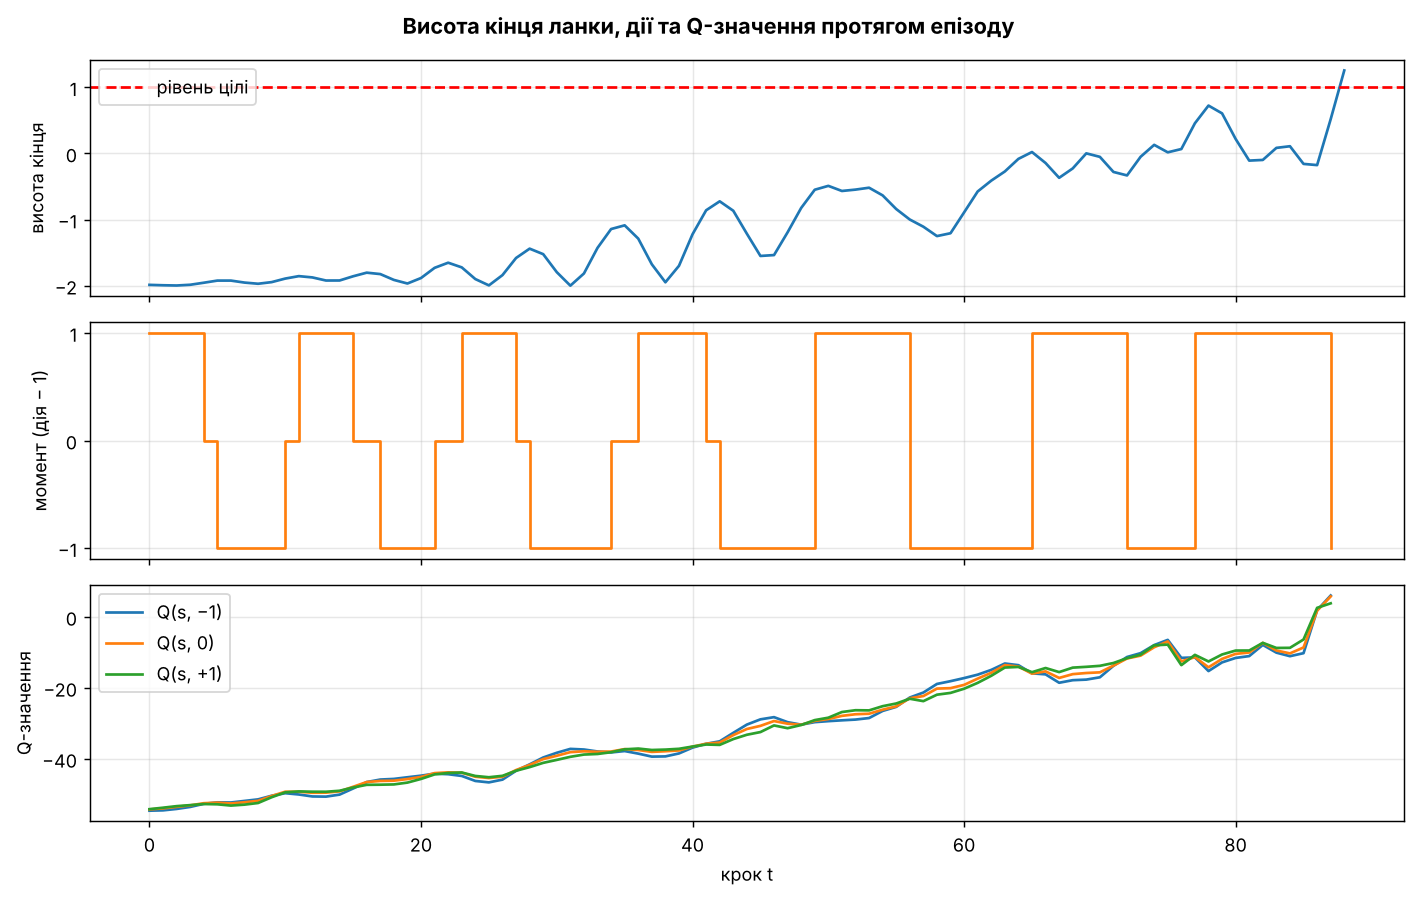
\includegraphics[width=0.92\textwidth]{../fig_episode.png}
\caption{Висота кінця нижньої ланки, вибрані дії та Q-значення протягом епізоду.}\label{fig:episode}
\end{figure}

Агент реалізує стратегію типу «bang-bang»: майже завжди максимальний момент $\pm1$ (42\,\% і 47\,\% кроків, нульовий момент — 11\,\%), напрям якого змінюється синхронно з коливанням маятника. Енергія системи накопичується, амплітуда висоти монотонно зростає (рис.~\ref{fig:episode}), і на 88-му кроці кінець ланки перетинає рівень цілі. Q-значення зростають від $-54$ до $\approx0$ в міру наближення до цілі, що узгоджується з їхнім змістом: $\max_aQ(s_0,a)=-54.2$ проти фактичного дисконтованого доходу $-(1-\gamma^{88})/(1-\gamma)=-58.7$ — невелика переоцінка, характерна для DQN через $\max$ у цілі. Криві трьох Q майже збігаються протягом усього епізоду — наочна ілюстрація малого action gap.

\section{Висновки}
\begin{enumerate}
\item Готова реалізація DQN (Stable-Baselines3) з гіперпараметрами RL Zoo стабільно розв'язує Acrobot-v1 за 60\,000 кроків: $-78.0\pm2.7$, 100\,\% успішних епізодів. Агент самостійно знаходить фізично осмислену стратегію накопичення енергії.
\item \textbf{Період оновлення цільової мережі} — найчутливіший параметр. Надто часте оновлення (10) прискорює початок, але робить навчання нестабільним. Надто рідке (2000) за обмежений бюджет унеможливлює навчання, бо цінності поширюються лише на один крок за кожне оновлення цілі.
\item \textbf{Крок навчання} у діапазоні $10^{-4}$–$3\cdot10^{-3}$ впливає переважно на швидкість і коливання, а не на кінцевий результат: Adam, функція Хубера та обрізання градієнта роблять метод стійким.
\item \textbf{Архітектура:} мережа [64,\,64] рівноцінна базовій за якістю і краща за швидкістю та стабільністю; [16] недостатня. Ємність потрібна насамперед для розрізнення близьких Q-значень дій.
\item \textbf{Дослідження:} базовий розклад (0.12, 0.1) найнадійніший; довше дослідження уповільнює старт, а мале кінцеве $\varepsilon$ підвищує ризик невдалого запуску.
\item Основний механізм невдач — \textbf{вироджена жадібна політика} через малий action gap. Звідси методичний висновок: якість DQN слід оцінювати детерміновано, на багатьох епізодах і кількох seed. Навчальні криві та окремі успішні епізоди можуть створювати хибне враження.
\end{enumerate}

\textbf{Обмеження дослідження.} 3 seed на конфігурацію: відмінності в кілька одиниць доходу статистично не значущі, надійно встановлено лише явні невдачі. Бюджет 60\,000 кроків замість 100\,000: повільні варіанти могли б покращитися. Проміжні оцінки за 10 епізодами шумні. Змінювався лише один гіперпараметр за раз, без їх взаємодій. Використано одне середовище. Час навчання вимірювався при паралельному завантаженні CPU і є орієнтовним.

\appendix
\section{Відповіді на контрольні запитання}
\begin{enumerate}[leftmargin=*]
\item \textbf{Off-policy}: ціль $\max_{a'}Q_{\theta^-}(s',a')$ відповідає жадібній політиці, а дані збирає $\varepsilon$-жадібна; тому можна навчатися на переходах, зібраних старішими версіями політики (буфер).
\item \textbf{Model-free}: використовуються лише переходи, отримані із середовища; модель $p(s'\mid s,a)$ не потрібна.
\item \textbf{Value-based}: навчається $Q_\theta$, політика визначається як $\arg\max_aQ_\theta$; окремої мережі політики немає.
\item Вектор із 6 неперервних чисел (cos/sin двох кутів і дві кутові швидкості), \code{Box(6,)}, float32.
\item 3 дискретні дії — момент $-1$, $0$, $+1$ Н·м у шарнірі між ланками.
\item $-1$ за кожен крок до досягнення цілі, $0$ на кроці досягнення. Заохочує досягати цілі якомога швидше; повністю відповідає меті, але розріджена.
\item \code{terminated} — кінець ланки вище рівня 1 (справжній кінець, майбутня цінність 0); \code{truncated} — 500 кроків (штучне обрізання, майбутня цінність не нульова).
\item Q-net (вхід — стан, виходи — $Q(s,a)$ трьох дій) і цільова Q-net тієї ж структури (для обчислення цілі).
\item Базова: 6$\to$256$\to$256$\to$3, ReLU у прихованих шарах, лінійний вихід. Замала мережа не розрізняє близькі Q (вироджена політика), надлишкова — повільніша без виграшу в якості.
\item $\varepsilon$-жадібно під час навчання ($\varepsilon$: 1$\to$0.1); при оцінюванні — детерміновано. Політика детермінована, стохастичність — лише дослідницький шум.
\item Переходи з буфера відтворення (50\,000 останніх); повторне використання можливе завдяки off-policy цілі.
\item Мінімізується функція Хубера між $Q_\theta(s,a)$ та ціллю $y$; кроки Adam за батчами з буфера, обрізання норми градієнта, періодичне копіювання ваг у цільову мережу.
\item \code{learning\_rate}, \code{buffer\_size}, \code{batch\_size}, \code{gamma}, \code{target\_update\_interval}, \code{train\_freq}/\code{gradient\_steps}, \code{learning\_starts}, \code{exploration\_fraction}, \code{exploration\_final\_eps}, \code{net\_arch} (див. табл. базової конфігурації).
\item Досліджено \code{learning\_rate}, \code{target\_update\_interval}, \code{net\_arch}, розклад $\varepsilon$. Гіпотези — розд.~5, спостереження — розд.~6. Несподіваними виявилися повна невдача target = 2000 і рівноцінність мережі [64,\,64] базовій.
\item У навчанні — $\varepsilon$-жадібний вибір і оновлення мережі; в оцінюванні — жадібний вибір без оновлень. Дії вибираються по-різному, тому якість політики треба вимірювати окремо.
\item Середній дохід і частка успіхів на 50 тестових епізодах, розкид між seed, крок досягнення порогу, коливання оцінок. Один епізод не показовий через стохастичність початкових станів і нестабільність навчання.
\item Використано \code{DQN}, \code{Monitor}, \code{EvalCallback} з SB3 і гіперпараметри RL Zoo. Самостійно — план і скрипт експериментів, оцінювання, діагностика, аналіз і візуалізація.
\item Див. розд.~7: найважливіші висновки стосуються цільової мережі, ємності мережі та необхідності детермінованого багатоепізодного оцінювання. Обмеження — кількість seed, бюджет кроків, одне середовище.
\end{enumerate}

\begin{thebibliography}{9}
\bibitem{mnih} V. Mnih et al. Human-level control through deep reinforcement learning. \emph{Nature}, 518:529–533, 2015.
\bibitem{sb3} A. Raffin et al. Stable-Baselines3: Reliable Reinforcement Learning Implementations. \emph{JMLR}, 22(268):1–8, 2021. \url{https://github.com/DLR-RM/stable-baselines3}
\bibitem{zoo} A. Raffin. RL Baselines3 Zoo. \url{https://github.com/DLR-RM/rl-baselines3-zoo}
\bibitem{gym} Gymnasium. Acrobot. \url{https://gymnasium.farama.org/environments/classic_control/acrobot/}
\bibitem{sutton} R. S. Sutton, A. G. Barto. \emph{Reinforcement Learning: An Introduction}, 2nd ed. MIT Press, 2018.
\end{thebibliography}

\end{document}
